% https://github.com/cohomolo-gy/cats-in-context/blob/master/chapter-2/Chapter%202%20Solutions.tex

\documentclass[14pt]{report}
\usepackage{bbm}
\usepackage{bbding} % for flower.
\usepackage{physics}
\usepackage{amsmath,amssymb}
\usepackage{graphicx}
\usepackage{makeidx}
\usepackage{algpseudocode}
\usepackage{algorithm}
\usepackage{listing}
\usepackage{minted}
\usemintedstyle{perldoc}
\usepackage{quiver}
\usepackage{enumitem}
\usepackage{mathtools}

\usepackage{xargs}



\usepackage{hyperref}
\hypersetup{
    colorlinks,
    citecolor=blue,
    filecolor=blue,
    linkcolor=blue,
    urlcolor=blue
}

\usepackage{epsfig}
\usepackage{tabularx}
\usepackage{latexsym}
\newcommand{\N}{\ensuremath{\mathbb{N}}}
\newcommand{\Z}{\ensuremath{\mathbb{Z}}}
\newcommand{\Q}{\ensuremath{\mathbb{Q}}}
\newcommand{\R}{\ensuremath{\mathbb R}}

\def\qed{\ensuremath{\Box}}

\newcommand*{\start}[1]{\leavevmode\newline \textbf{#1} }
\newcommand*{\question}[1]{\leavevmode\newline \textbf{Question: #1.}}
\newcommand*{\proof}[1]{\leavevmode\newline \textbf{Proof #1}}
\newcommand*{\answer}{\leavevmode\newline \textbf{Answer} }
\DeclareMathOperator{\lcm}{lcm}


\usepackage[adobe-utopia]{mathdesign}
\usepackage[T1]{fontenc}

\title{Competitive programming proofs}
\author{Siddharth Bhat}
\date{Monsoon, second year of the plague}


\begin{document}
\maketitle
\tableofcontents

\chapter{Codeforces Problems}

\section{Codeforces 1389C: woodcutters}
Problem link is \url{https://codeforces.com/problemset/problem/1389/C}.
\begin{itemize}
\item Solution is greedy.
\item It's hopefully clear that it's always optimal to have the
    first tree lean left and the last tree lean right.  So we now
    have the prove that the construction for trees `[1..n-2]` is
    optimal.

\item Let $O_*$ be the optimal solution, $O$ be the solution discovered by the
    above algorithm.  Let index $i$ be the first index where $O_*$ and $O$
        decide to do something different to a tree.  We have $i > 0, i < n-2$
        since we assume that the algorithms agree on the first and last tree.
\item We have  6 cases at index `i`: the possibilities are `L` for leaning left, `U` for standing up, and `R` for leaning right.
\begin{itemize}
\item  $O_*=L, O=U$: If there is enough space to lean left, $O$ will choose to
    lean left. This violates the construction of $O$.
\item  $O_*=L, O=R$: Same as above; If there is space to lean left, $O$ will
    choose to lean left. This violates the construction of $O$.
\item  $O_*=U, O=L$: Since $O$ and $O_*$ agree upto $i$ and $O$ chooses to lean
    left, there must be enough space to lean left for $O_*$. This creates a
        strictly better solution,  which violates the optimality of $O_*$.
\item $O_*=U, O=R$: Now what? we can't control $O$ based on $O_*$ or vice
    versa.  We'll return to this case at the end, as it's the most complex.
\item $O_*=R, O=L$: There must be enough space for $O_*$ to lean $L$. $O_*=R$
    only limits the space available for the next tree. So we can modify $O_*$
        to lean left and reach the same optimality.
\item $O_*=R, O=U$: If it's possible to lean right, then $O$ will choose to do
    so. This violates the construction of $O$.
\end{itemize}

\item $O_*=U, O=R$: This is the complex case.
    \begin{itemize}
            \item In this case, let's consider the sequence of trees felled by $O_*$ after $i$.
            \item Let us suppose that $O_*$ fells many trees rightward,
                followed by a tree that is felled in the direction $d_*$ (where
                $d_* \in \{L, U \} \neq R$.  Formally, $O_*[i, i+1, k] = U; R^k; d_*$ for
                some $d_* \neq R$. (That is, $d_* \equiv O_*[k]$).
            \item If such a $d_O$ does not exist, then $O$ can
                mimic what $O_*$ does, since $O$'s decision to move $O[i]$ right does not impact any tree in the future.
            \item If such a $d_*$ does exist, then let us consider what $d_*$ is.
            \item If $d_* \equiv O_*[k]$ is $U$, then we can have $O[k] = U$.
            \item If $d_* \equiv O_*[k]$ is $L$, then we can have $O[k] = U$.
    \end{itemize}
\end{itemize}

\newpage

\section{Codeforces  1175 C: Electrification}

sliding window argument.

I will proof this by a simple contradiction argument Assume that at least one of the N nearest neighbours of x does not belong to a continuous window of size N containing x. Let us assume this nearest neighbour is Aj. Without loss of generality, assume Aj<x (same proof works for Aj>x). As the window is not continuous as per our assumption, there must exist some element Ak between Aj and x which is not a nearest neighbour of x. But distance of Ak from x is clearly less than distance of Aj from x. So if Aj is a nearest neighbour, Ak must also be a nearest neighbour. That contradicts our assumption.


\newpage


\section{Codeforces 190D: Non-Secret Cypher}

\begin{quote}{Yeputons}
It's kind of optimization. Consider problem \href{https://codeforces.com/contest/190/problem/D}{190D - Non-Secret Cypher}. The
stupid solution goes over all subarrays and checks whether it's good or
not. Now we notice that if subarray is 'good', then all its superarrays is
'good' too. Let's go over all left borders $1 \leq x \leq N$
and for each of them find $r_x$. rx is a minimal number such that subarray
$x \dots  r_x$ is good.  Obviously, all subarrays which starts at $x$ and
ends after $r_x$ is good.  If you notice that $r_1 \leq r_2 \leq \dots \leq r_N$,
you can use 'two pointers' method. The first pointer is $x$ and the second one
is $r_x$. When you move the first one right, the second one
\emph{can only move right} too. No matter how many operations you perform in one step,
algo's running time is $O(n)$, because each of pointers makes $\leq N$
steps.
\end{quote}

\newpage


\section{Codeforces 1389C:}
\begin{itemize}
\item It's safe to look for a longest satisfying match with DP, and if the
    match is of odd length, to decrement it to get an even length string.
\item This would NOT be safe if we had to chop of an arbitrary length $\delta$!
    \begin{itemize}
        \item To instill fear, suppose $\delta = 5$,
            and that on some problem instance, the best string had length $9$, second best had length $7$.
        \item Since the DP only keeps track of the longest length, we would
            have tracked $9$, and then subtracted $5$ to report $9-5=4$ which
            is much less than the real second-optima of $7$.
    \end{itemize}
\item The reason this is safe when we chop off length $1$ is because:
    \begin{itemize}
            \item We already know that, say, $9$ is the longest string length.
                There are no longer solutions that can compete. So we can must
                only worry about shorter solutions
            \item Amongst the second largest solutions, we must worry about the second largest solution being $8, 7, 6, \dots$.
            \item Since we only decrement by $1$, our "mutated" largest solutoin will be $8$. This is as large as the
                maximum second-largest solution.
            \item So we do not lost any second-best optima, since we mutate the first best optima to drop by $1$, which makes it
                the best-in-class second best optima.
    \end{itemize}
\end{itemize}

% https://www.baeldung.com/cs/sliding-window-algorithm
\section{Codeforces 676C: Vasya and String}
\begin{itemize}
    \item Problem link: \url{https://codeforces.com/contest/676/problem/C}
    \item Here, we learn how to write a proof of correctness for sliding window where the window length is \emph{upper bounded}. That is,
        we have a \emph{maximum} length of sliding window that we cannot exceed.
    \item \emph{Key Idea 1}: consider all windows that contain legal solutions. Suppose we have two windows $[l_1, r_1]$ and $[l_2, r_2]$
        where $r_1 < r_2$ (that is, window $1$ ends before window $2$). Then, we wish to show that $l_1 < l_2$ (that is, window $1$
        begins before window $2$).
    \item This condition implies that when we make progress by moving $r_1 \rightarrow r_2$, we can similarly make forward progress
      moving $l_1 \rightarrow l_2$. We would not have to go backwards, like
      $l_2 \leftarrow l_1$.  So when we move from $r$ to $(r+1)$, we need to
      decide how much we must move $l$. We know that this will not lose
      solutions from the prior invariant.
\end{itemize}


Let's consider a simpler subproblem, where are given a string of \texttt{'a'}s and \texttt{'b'}s and we must find
the longest substring with at most $k$ \texttt{'b'}s. The original problem can be solved by solving this problem twice,
once with \texttt{'a, b'} and once by swapping these letters.

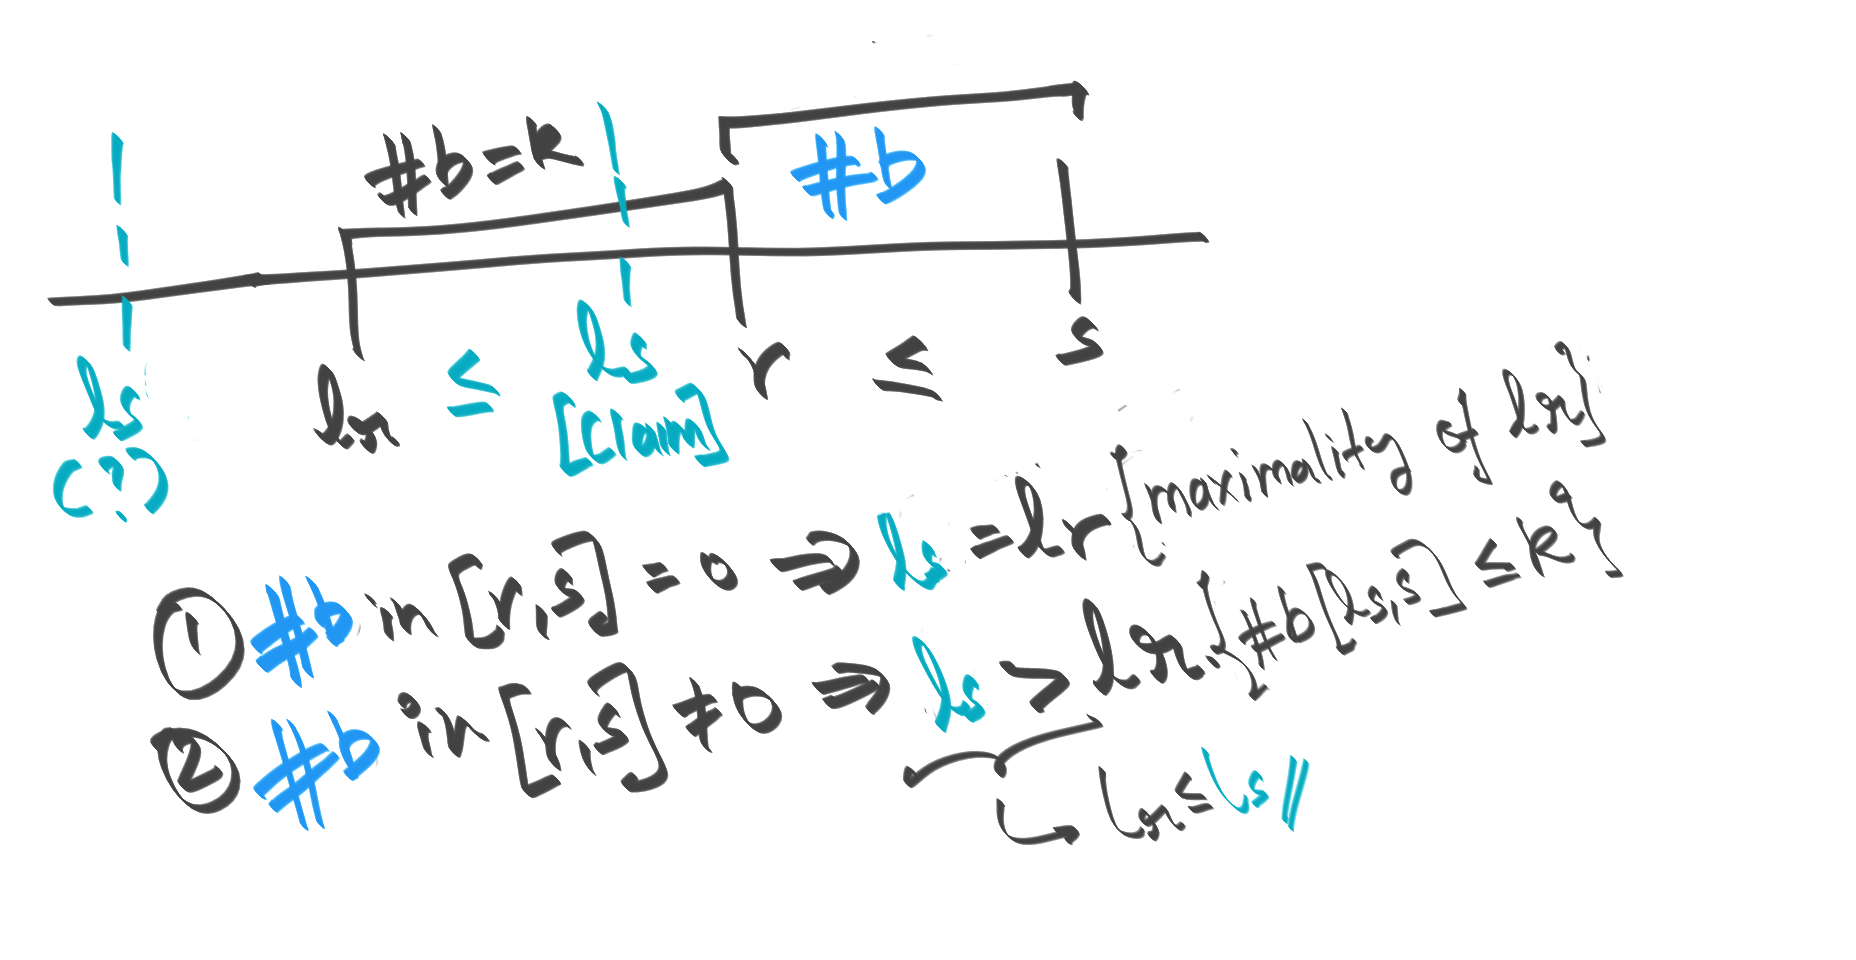
\includegraphics[width=\textwidth]{problems/676c/sliding-window-optimality.png}

\begin{itemize}
    \item At this subproblem, let us have $r \leq s$. We wish to show that $l_r \leq l_s$, where $l_x$ 
        is the leftmost index such that $[l_x \dots x]$ is a legal index. We begin by case analysis on the number of \texttt{'b'}s
        in the interval $[r, s]$.
    \item (a) zero \texttt{'b'}s in $[r, s]$: Then we claim that $l_s \geq l_r$ (In fact, $l_s = l_r)$. Suppose $l_s < l_r$.
        This means that the interval $[l_s < l_r \leq r \leq s]$ contains at most $k$ \texttt{'b'}s. Thus, the interval $[l_s < \l_r \leq r]$
        also contains at most $k$ \texttt{'b'}s. But this contradicts the maximality of the value $l_r$. Hence, $l_s \geq l_r$.
        This implies that $r \leq s \implies l_r \leq l_s$.
    \item (b) one or more \texttt{'b'}s in $[r, s]$. Then we claim that $l_s > l_r$. Suppose $l_s \leq l_r$.
        Since $l_r$ was maximal, we have either (b1) The interval $[l_r \dots r]$ has $k$ \texttt{'b'}s ($#b(s[l_r, \dots, r]) = k$)
        or (b2) $l_r$ is the leftmost index ($l_r = 1$ and $#b(s[l_r, \dots, r] < k$).
        \begin{itemize}
            \item (b1) in this case, we must have $l_s \geq l_r$. Suppose not. Then we have that $l_s < l_r < r < s$. So the interval
                $[l_r, r]$ is strictly contained in $[l_s, r]$ (which is also a legal interval). This contradicts the maximality of $l_r$.
            \item (b2) $l_r$ is the leftmost index possible, so we trivially have $l_r \leq l_s$.
        \end{itemize}
\end{itemize}

\begin{minted}{cpp}
// https://codeforces.com/contest/676/submission/121164663
void main() {
  ...
  int best = 0;
  for (int c = 'a'; c <= 'b'; ++c) {
    int l = 0;
    int changed = 0;
    // [l, r]
    for (int r = 0; r < n; ++r) {
      // change to c
      if (s[r] != c) { changed++; }
      while (changed > k) {
          if (s[l] != c) { changed--; }
          l++;
      }
      best = max(best, r - l + 1);
    }
  }
  cout << best;
}
\end{minted}



% https://www.baeldung.com/cs/sliding-window-algorithm
\section{Codeforces 676C: Vasya and String}
\begin{itemize}
    \item Problem link: \url{https://codeforces.com/contest/676/problem/C}
    \item Here, we learn how to write a proof of correctness for sliding window where the window length is \emph{upper bounded}. That is,
        we have a \emph{maximum} length of sliding window that we cannot exceed.
    \item \emph{Key Idea 1}: consider all windows that contain legal solutions. Suppose we have two windows $[l_1, r_1]$ and $[l_2, r_2]$
        where $r_1 < r_2$ (that is, window $1$ ends before window $2$). Then, we wish to show that $l_1 < l_2$ (that is, window $1$
        begins before window $2$).
    \item This condition implies that when we make progress by moving $r_1 \rightarrow r_2$, we can similarly make forward progress
      moving $l_1 \rightarrow l_2$. We would not have to go backwards, like
      $l_2 \leftarrow l_1$.  So when we move from $r$ to $(r+1)$, we need to
      decide how much we must move $l$. We know that this will not lose
      solutions from the prior invariant.
\end{itemize}


Let's consider a simpler subproblem, where are given a string of \texttt{'a'}s and \texttt{'b'}s and we must find
the longest substring with at most $k$ \texttt{'b'}s. The original problem can be solved by solving this problem twice,
once with \texttt{'a, b'} and once by swapping these letters.

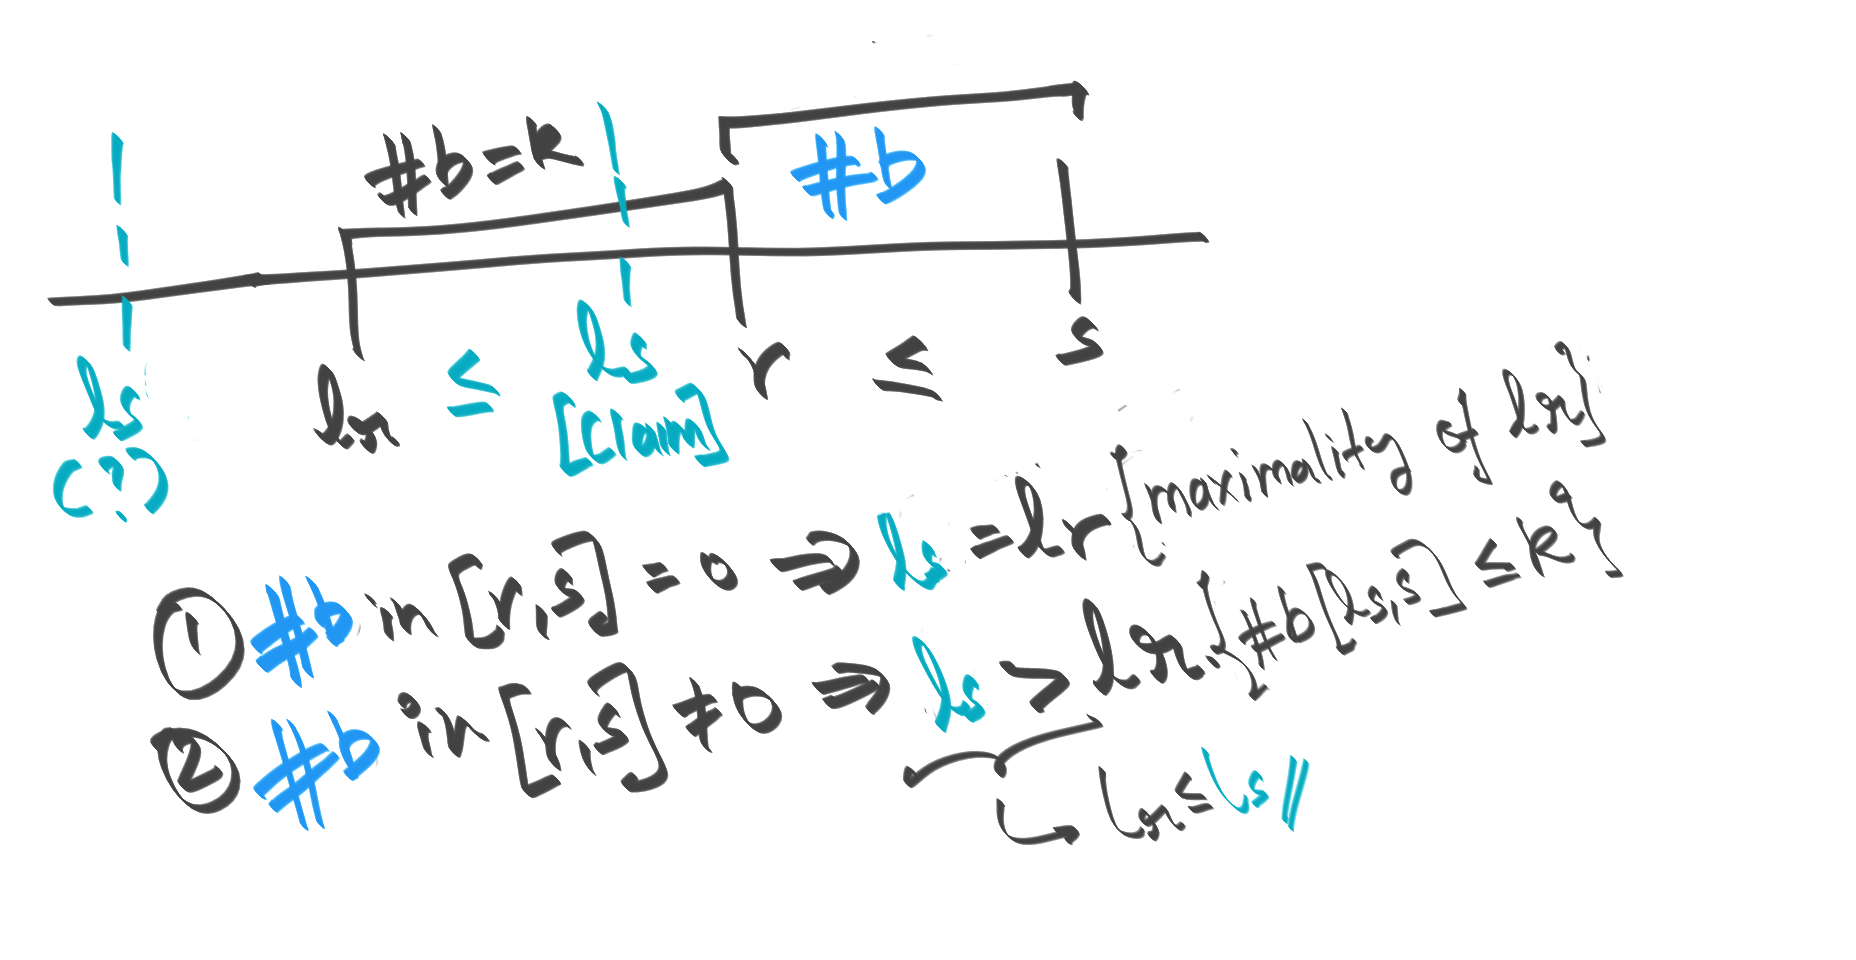
\includegraphics[width=\textwidth]{problems/676c/sliding-window-optimality.png}

\begin{itemize}
    \item At this subproblem, let us have $r \leq s$. We wish to show that $l_r \leq l_s$, where $l_x$ 
        is the leftmost index such that $[l_x \dots x]$ is a legal index. We begin by case analysis on the number of \texttt{'b'}s
        in the interval $[r, s]$.
    \item (a) zero \texttt{'b'}s in $[r, s]$: Then we claim that $l_s \geq l_r$ (In fact, $l_s = l_r)$. Suppose $l_s < l_r$.
        This means that the interval $[l_s < l_r \leq r \leq s]$ contains at most $k$ \texttt{'b'}s. Thus, the interval $[l_s < \l_r \leq r]$
        also contains at most $k$ \texttt{'b'}s. But this contradicts the maximality of the value $l_r$. Hence, $l_s \geq l_r$.
        This implies that $r \leq s \implies l_r \leq l_s$.
    \item (b) one or more \texttt{'b'}s in $[r, s]$. Then we claim that $l_s > l_r$. Suppose $l_s \leq l_r$.
        Since $l_r$ was maximal, we have either (b1) The interval $[l_r \dots r]$ has $k$ \texttt{'b'}s ($#b(s[l_r, \dots, r]) = k$)
        or (b2) $l_r$ is the leftmost index ($l_r = 1$ and $#b(s[l_r, \dots, r] < k$).
        \begin{itemize}
            \item (b1) in this case, we must have $l_s \geq l_r$. Suppose not. Then we have that $l_s < l_r < r < s$. So the interval
                $[l_r, r]$ is strictly contained in $[l_s, r]$ (which is also a legal interval). This contradicts the maximality of $l_r$.
            \item (b2) $l_r$ is the leftmost index possible, so we trivially have $l_r \leq l_s$.
        \end{itemize}
\end{itemize}

\begin{minted}{cpp}
// https://codeforces.com/contest/676/submission/121164663
void main() {
  ...
  int best = 0;
  for (int c = 'a'; c <= 'b'; ++c) {
    int l = 0;
    int changed = 0;
    // [l, r]
    for (int r = 0; r < n; ++r) {
      // change to c
      if (s[r] != c) { changed++; }
      while (changed > k) {
          if (s[l] != c) { changed--; }
          l++;
      }
      best = max(best, r - l + 1);
    }
  }
  cout << best;
}
\end{minted}



% https://www.baeldung.com/cs/sliding-window-algorithm
\section{Codeforces 676C: Vasya and String}
\begin{itemize}
    \item Problem link: \url{https://codeforces.com/contest/676/problem/C}
    \item Here, we learn how to write a proof of correctness for sliding window where the window length is \emph{upper bounded}. That is,
        we have a \emph{maximum} length of sliding window that we cannot exceed.
    \item \emph{Key Idea 1}: consider all windows that contain legal solutions. Suppose we have two windows $[l_1, r_1]$ and $[l_2, r_2]$
        where $r_1 < r_2$ (that is, window $1$ ends before window $2$). Then, we wish to show that $l_1 < l_2$ (that is, window $1$
        begins before window $2$).
    \item This condition implies that when we make progress by moving $r_1 \rightarrow r_2$, we can similarly make forward progress
      moving $l_1 \rightarrow l_2$. We would not have to go backwards, like
      $l_2 \leftarrow l_1$.  So when we move from $r$ to $(r+1)$, we need to
      decide how much we must move $l$. We know that this will not lose
      solutions from the prior invariant.
\end{itemize}


Let's consider a simpler subproblem, where are given a string of \texttt{'a'}s and \texttt{'b'}s and we must find
the longest substring with at most $k$ \texttt{'b'}s. The original problem can be solved by solving this problem twice,
once with \texttt{'a, b'} and once by swapping these letters.

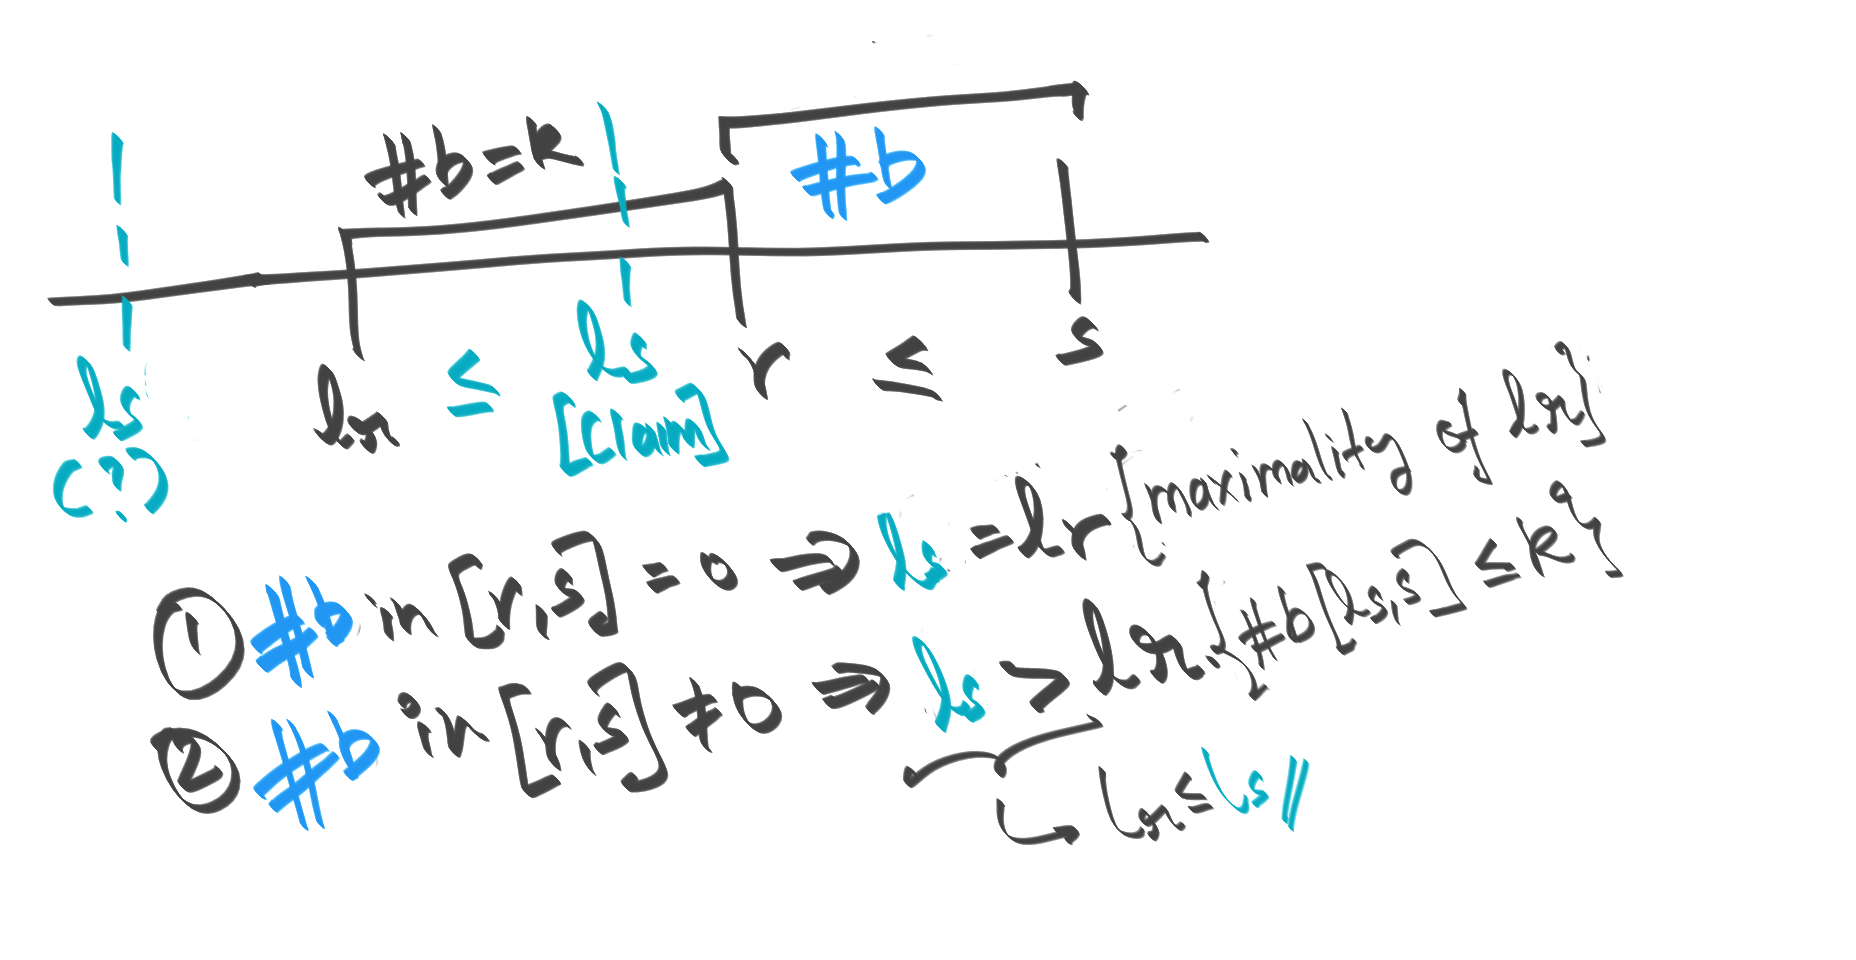
\includegraphics[width=\textwidth]{problems/676c/sliding-window-optimality.png}

\begin{itemize}
    \item At this subproblem, let us have $r \leq s$. We wish to show that $l_r \leq l_s$, where $l_x$ 
        is the leftmost index such that $[l_x \dots x]$ is a legal index. We begin by case analysis on the number of \texttt{'b'}s
        in the interval $[r, s]$.
    \item (a) zero \texttt{'b'}s in $[r, s]$: Then we claim that $l_s \geq l_r$ (In fact, $l_s = l_r)$. Suppose $l_s < l_r$.
        This means that the interval $[l_s < l_r \leq r \leq s]$ contains at most $k$ \texttt{'b'}s. Thus, the interval $[l_s < \l_r \leq r]$
        also contains at most $k$ \texttt{'b'}s. But this contradicts the maximality of the value $l_r$. Hence, $l_s \geq l_r$.
        This implies that $r \leq s \implies l_r \leq l_s$.
    \item (b) one or more \texttt{'b'}s in $[r, s]$. Then we claim that $l_s > l_r$. Suppose $l_s \leq l_r$.
        Since $l_r$ was maximal, we have either (b1) The interval $[l_r \dots r]$ has $k$ \texttt{'b'}s ($#b(s[l_r, \dots, r]) = k$)
        or (b2) $l_r$ is the leftmost index ($l_r = 1$ and $#b(s[l_r, \dots, r] < k$).
        \begin{itemize}
            \item (b1) in this case, we must have $l_s \geq l_r$. Suppose not. Then we have that $l_s < l_r < r < s$. So the interval
                $[l_r, r]$ is strictly contained in $[l_s, r]$ (which is also a legal interval). This contradicts the maximality of $l_r$.
            \item (b2) $l_r$ is the leftmost index possible, so we trivially have $l_r \leq l_s$.
        \end{itemize}
\end{itemize}

\begin{minted}{cpp}
// https://codeforces.com/contest/676/submission/121164663
void main() {
  ...
  int best = 0;
  for (int c = 'a'; c <= 'b'; ++c) {
    int l = 0;
    int changed = 0;
    // [l, r]
    for (int r = 0; r < n; ++r) {
      // change to c
      if (s[r] != c) { changed++; }
      while (changed > k) {
          if (s[l] != c) { changed--; }
          l++;
      }
      best = max(best, r - l + 1);
    }
  }
  cout << best;
}
\end{minted}



% https://www.baeldung.com/cs/sliding-window-algorithm
\section{Codeforces 676C: Vasya and String}
\begin{itemize}
    \item Problem link: \url{https://codeforces.com/contest/676/problem/C}
    \item Here, we learn how to write a proof of correctness for sliding window where the window length is \emph{upper bounded}. That is,
        we have a \emph{maximum} length of sliding window that we cannot exceed.
    \item \emph{Key Idea 1}: consider all windows that contain legal solutions. Suppose we have two windows $[l_1, r_1]$ and $[l_2, r_2]$
        where $r_1 < r_2$ (that is, window $1$ ends before window $2$). Then, we wish to show that $l_1 < l_2$ (that is, window $1$
        begins before window $2$).
    \item This condition implies that when we make progress by moving $r_1 \rightarrow r_2$, we can similarly make forward progress
      moving $l_1 \rightarrow l_2$. We would not have to go backwards, like
      $l_2 \leftarrow l_1$.  So when we move from $r$ to $(r+1)$, we need to
      decide how much we must move $l$. We know that this will not lose
      solutions from the prior invariant.
\end{itemize}


Let's consider a simpler subproblem, where are given a string of \texttt{'a'}s and \texttt{'b'}s and we must find
the longest substring with at most $k$ \texttt{'b'}s. The original problem can be solved by solving this problem twice,
once with \texttt{'a, b'} and once by swapping these letters.

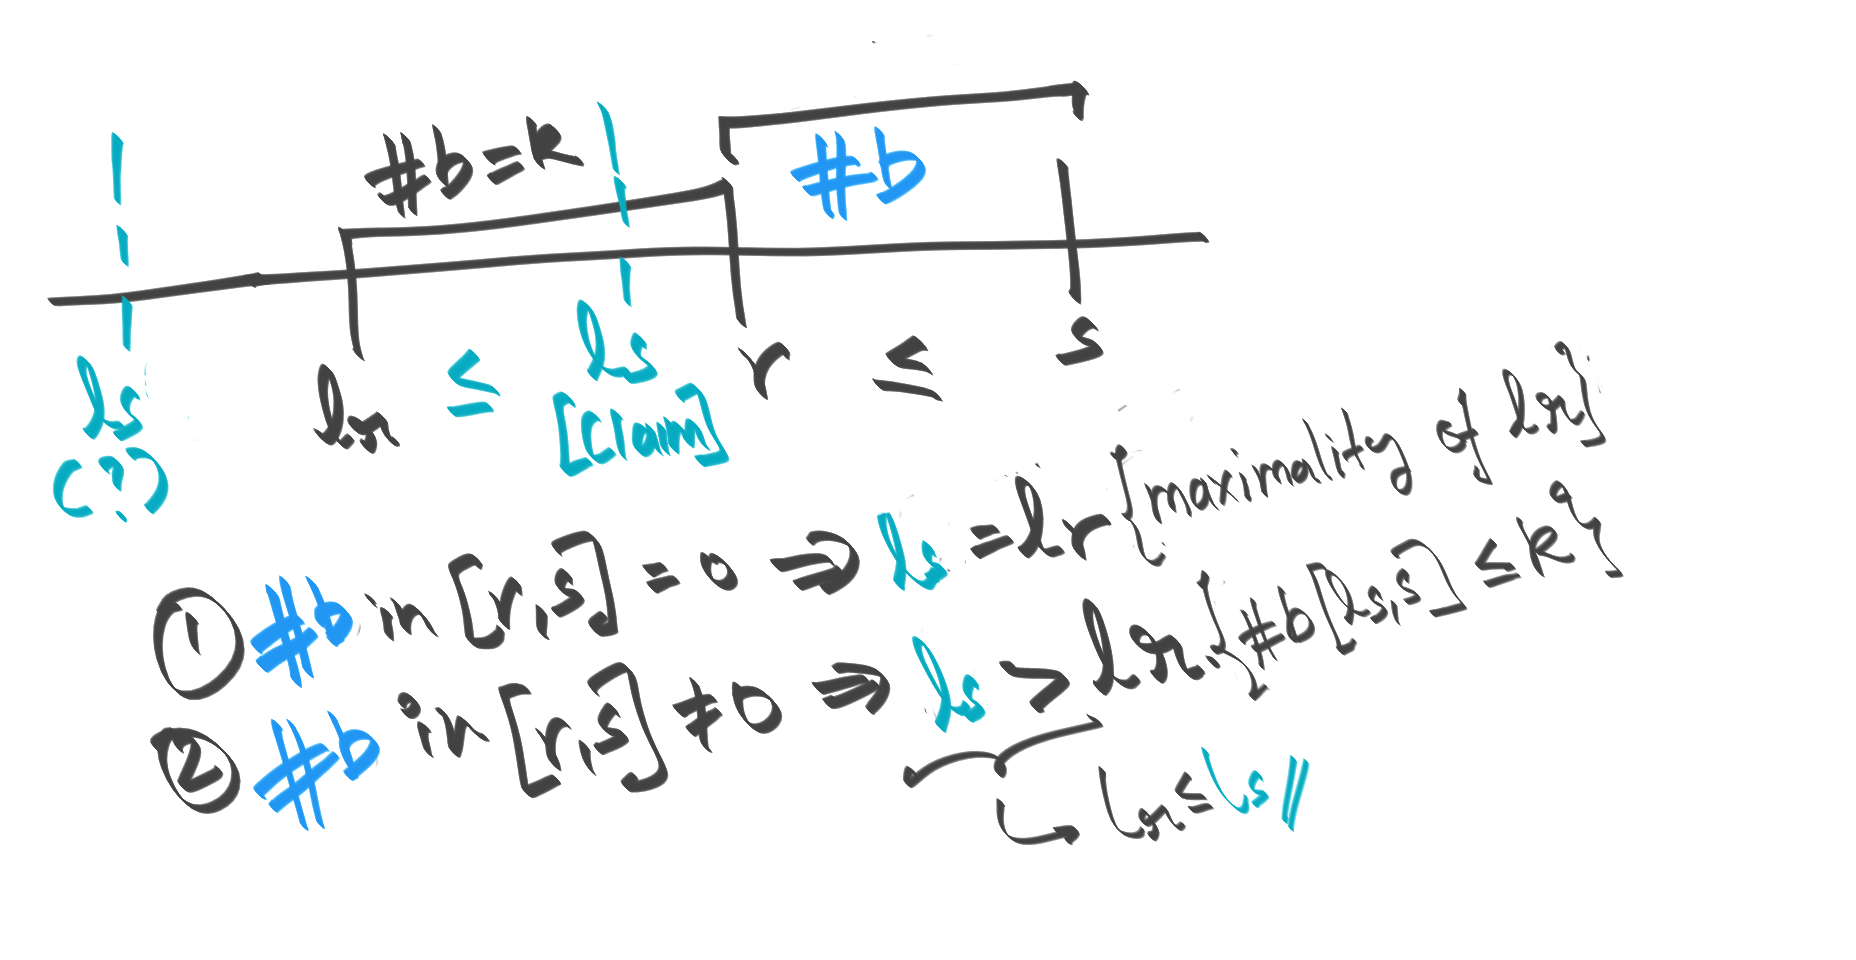
\includegraphics[width=\textwidth]{problems/676c/sliding-window-optimality.png}

\begin{itemize}
    \item At this subproblem, let us have $r \leq s$. We wish to show that $l_r \leq l_s$, where $l_x$ 
        is the leftmost index such that $[l_x \dots x]$ is a legal index. We begin by case analysis on the number of \texttt{'b'}s
        in the interval $[r, s]$.
    \item (a) zero \texttt{'b'}s in $[r, s]$: Then we claim that $l_s \geq l_r$ (In fact, $l_s = l_r)$. Suppose $l_s < l_r$.
        This means that the interval $[l_s < l_r \leq r \leq s]$ contains at most $k$ \texttt{'b'}s. Thus, the interval $[l_s < \l_r \leq r]$
        also contains at most $k$ \texttt{'b'}s. But this contradicts the maximality of the value $l_r$. Hence, $l_s \geq l_r$.
        This implies that $r \leq s \implies l_r \leq l_s$.
    \item (b) one or more \texttt{'b'}s in $[r, s]$. Then we claim that $l_s > l_r$. Suppose $l_s \leq l_r$.
        Since $l_r$ was maximal, we have either (b1) The interval $[l_r \dots r]$ has $k$ \texttt{'b'}s ($#b(s[l_r, \dots, r]) = k$)
        or (b2) $l_r$ is the leftmost index ($l_r = 1$ and $#b(s[l_r, \dots, r] < k$).
        \begin{itemize}
            \item (b1) in this case, we must have $l_s \geq l_r$. Suppose not. Then we have that $l_s < l_r < r < s$. So the interval
                $[l_r, r]$ is strictly contained in $[l_s, r]$ (which is also a legal interval). This contradicts the maximality of $l_r$.
            \item (b2) $l_r$ is the leftmost index possible, so we trivially have $l_r \leq l_s$.
        \end{itemize}
\end{itemize}

\begin{minted}{cpp}
// https://codeforces.com/contest/676/submission/121164663
void main() {
  ...
  int best = 0;
  for (int c = 'a'; c <= 'b'; ++c) {
    int l = 0;
    int changed = 0;
    // [l, r]
    for (int r = 0; r < n; ++r) {
      // change to c
      if (s[r] != c) { changed++; }
      while (changed > k) {
          if (s[l] != c) { changed--; }
          l++;
      }
      best = max(best, r - l + 1);
    }
  }
  cout << best;
}
\end{minted}





\newpage

\section{Codeforces 1546D}

\begin{align*}
&f[p, m] = f[p-1, m-2] + f[p, m-1] \\
&\sum_{p\geq 1, m \geq 2}f[p, m] = \sum_{p \geq 1, m \geq 2} f[p-1, m-2] + f[p, m-1] \\
&\sum_{p\geq 1, m \geq 2}f[p, m] = \sum_{p \geq 1, m \geq 2} f[p-1, m-2] + f[p, m-1] \\
\end{align*}

\begin{minted}{text}
   |          |
--(+-p0, m0)-(+-p0, m1)-(- p0, m2)-(- p0, m3)-(- p0, m4)-> f[p=0,m]
  (| p1, m0) (| p1, m1) (* p1, m2) (* p1, m3) (* p1, m4)
  (| p2, m0) (| p2, m1) (* p2, m2) (* p2, m3) (* p2, m4)
  (| p3, m0) (| p3, m1) (* p3, m2) (* p3, m3) (* p3, m4)
  (| p4, m0) (| p4, m1) (* p4, m2) (* p4, m3) (* p4, m4)
  (| p5, m0) (| p5, m1) (* p5, m2) (* p5, m3) (* p5, m4)
   |          |                                         f[p>=1, m>=2]
   v          v
  f[m=0,p]    f[m=1,p]
\end{minted}

Let $g(x, y) \equiv \sum_{p \geq 0, m \geq 0} f(p, m) x^p y^m$ be the generating function for $f$.

{\footnotesize
\begin{align*}
&\sum_{p\geq 1, m \geq 2}f[p, m] x^p y^m \\
&= g(x, y) - \sum f[p=0, m \geq 0] x^py^m - \sum f[p \geq 0, m=0] x^p y^m - \sum f[p \geq 0, m = 1] x^p y^m + \sum f[p=0, m=0] + f[p=0, m=1] \\
&= g(x, y) - \sum_{p=0, m \geq 0} f[p, m] x^py^m - \sum_{p\geq 0, m = 0} f[p, m] x^py^m  - \sum_{p \geq 0, m = 1} f[p, m] x^py^m + f[p:0,m:0] + f[p:0, m:1] y \\
&= g(x, y) - \sum_{p=0, m \geq 0} f[p, m] x^py^m - \sum_{p\geq 0, m = 0} f[p, m] x^py^m  - \sum_{p \geq 0, m = 1} f[p, m] x^py^m + f[p:0,m:0] + f[p:0, m:1] y \\
&= g(x, y) - \sum_{m \geq 0} f[p=0, m] x^py^m - \sum_{p\geq 0} f[p, m=0] x^py^m  - \sum_{p \geq 0} f[p, m=1] x^py^m + f[p=0,m=0] + f[p:0, m=1] y \\
&= g(x, y) - \sum_{m \geq 0} (f[p=0, m] = 1)y^m - \sum_{p\geq 0} (f[p, m=0] = \delta_0^p) x^p  - \sum_{p \geq 0} (f[p, m=1] = \delta_0^p) x^py + f[p=0,m=0] + f[p:0, m=1] y \\
&= g(x, y) - 1/(1-y) - 1  - y + 1 + y \\
&= g(x, y) - 1/(1-y)  \\
\end{align*}
}

(take pairwise intersection of summations. $(p=0, m \geq 0) \cap  (p=1, m \geq 0) = \emptyset$, $(p = 0, m \geq 0) \cap (m = 0, p \geq 0) = (p:0, m:0)$ and so on.

\begin{align*}
&\sum_{p \geq 1, m \geq 2} f[p-1, m-2] x^p y^m
&= xy^2 \sum_{p \geq 2, m \geq 1} f[p-1, m-2] x^{p-1} y^{m-2} = xy^2 g(x, y)
\end{align*}

\begin{align*}
&\sum_{p \geq 1, m \geq 2} f[p, m-1] x^p y^m      \\
&= y \sum_{p \geq 1, m \geq 2} f[p, m-1] x^p y^{m-1} \\
&= y \sum_{p \geq 1, m' \geq 1} f[p, m'] x^p y^{m'} \\
&= y \left( g(x, y) - \sum_{p\geq 0} f[p, m'=0]x^p - \sum_{m' \geq 0} f[p=0, m']y^{m'} + f(p=0, m=0) \right) \\
&= y \left( g(x, y) - \sum_{p\geq 0} (f[p, m'=0] = \delta_p^0 )x^p  - \sum_{m' \geq 0} (f[p=0, m']=1) \cdot y^{m'} + (f(p=0, m=0)=1) \right) \\
&= y \left( g(x, y) - x^0  - 1/(1-y) + 1 \right) \\
&= y g(x, y) - y/(1-y)  \\
\end{align*}

This means the recurrence is:

\begin{align*}
&f[p, m] = f[p-1, m-2] + f[p, m-1] \\
&g(x, y) - 1/(1-y) =  \left [ xy^2 g(x, y)  \right] +  \left[ y g(x, y) - y/(1-y) \right] \\
&g(x, y) \left( 1 - xy^2 - y\right) = -y(1-y) + 1/(1-y) \\
&g(x, y) \left( 1 - xy^2 - y\right) = (1-y)/(1-y) = 1 \\
&g(x, y) = \frac{1}{1 - (xy^2 + y)} = \frac{1}{(1 - y) - xy^2} \\
&g(x, y) = \frac{1}{1 - y} \left( \frac{1}{1 - \left ( \frac{y^2}{1 - y} \right) \times x} \right) \\
&g(x, y) = \frac{1}{1-y} \left ( \sum_{p \geq 0} x^p {y^{2p}}{(1-y)^{-p}}  \right)    \\
&g(x, y) = \sum_{p \geq 0} x^p {y^{2p}}{(1-y)^{-(p+1)}} \\
&g(x, y) = \sum_{p \geq 0} x^p {y^{2p}}\sum_{j=0}^\infty \binom{(p+1)+j-1}{j}y^j  \\
&g(x, y) = \sum_{p \geq 0}\sum_{j=0}^\infty  x^p \binom{p+j}{j}y^{2p+j}  \\
\end{align*}

Sidenote: we count the coefficient of $y^j$ in $(1-y)^{-(p+1)}$ using stars and bars: the expression
expands into $(1 + y + y^2 + \dots)^{-(p+1)}$ so we have $j$ objects (copies of $y$ in $y^j$) and we have $(p+1)$ bars
(which copies of $y$ come from which term of $(1 - y)^{-(p+1)}$.

Let $m = 2p + j$. $p$ is fixed by the summation, so we have $j = m-2p$.

\begin{align*}
&g(x, y) = \sum_{p \geq 0}\sum_{j\geq 0} x^p \binom{p+j}{j}y^{2p+j}  \\
&g(x, y) = \sum_{p \geq 0}\sum_{j\geq 0} x^p \binom{p+(m-2p)}{j}y^{2p+(m-2p)}  \\
&g(x, y) = \sum_{p \geq 0}\sum_{j\geq 0} x^p \binom{m-p}{m-2p}y^{m}  \\
&g(x, y) = \sum_{p \geq 0}\sum_{j\geq 0} x^p \binom{m-p}{(m - p) - (m-2p)}y^{m}  \\
&g(x, y) = \sum_{p \geq 0}\sum_{j\geq 0} x^p \binom{m-p}{p}y^{m}  \\
\end{align*}


So the solution is $f(m, p) \equiv \binom{m-p}{p}$.

We have a $1 \times n$ chessboard and $p$ $1x2$ tiles. So treat the $p$ tiles as one kind of object and then $(n-2p)$ spaces
as another kind of object. How many arrangements of these are there? ($(p + n - 2p)!/p!(n-2p)! = \binom{n-p}{p}$).

In the combinatorial interpretation, we shrink the $1\times 2$ tiles also into $1 \times 1$ tiles.
This causes us to lose $p$ spaces. Out of these $(n-p)$ leftover locations, we choose $p$ locations
for the tiles.

\section{Codeforces  ?: Minimise sum of absolute differences while preserving total}

Given a number $S$ create an array of non-negative ($\geq 0$) integers $a[i]$ of size $n$ such that $\sum_{0 \leq i < n} a[i] = S$,
which minimises $\delta \equiv \sum_{i > j} | a[i] - a[j]|$.


\chapter{Combinatorial game theory}
% https://web.mit.edu/sp.268/www/nim.pdf
% https://www.youtube.com/watch?v=YV_oWBi1_ck&list=PLxYr6TaF_SDV5r6rmI0LDxuO48FPFb6Rk&index=3
\start{Definition: Normal rule} player with no moves left \emph{wins}.
\start{Definition: P position} player with no moves left \emph{loses}.

\start{Definition: P position} position that is winning for \emph{previous} player (last player who made a move).
\start{Definition: N position} position that is winning for \emph{next} player (player whose turn it is / player who will be making a move).

\start{Recursive definition of position under misere rule (eg. chess without stalemate)}
\begin{itemize}
    \item Terminal positions are P positions.
    \item From every N position, there is at least one move to a P position.
    \item from every P position, there is at least one move to an N position.
\end{itemize}
\end{document}

